\title{Dux: Automating Dependency Management}
\author{
        Martin Kellogg \\
        University of Washington
            \and
        Steven Lyubomirsky\\
        University of Washington
}


\documentclass[10pt,conference]{IEEEtran}

\usepackage{graphicx}
\graphicspath{ {images/} }
\usepackage{myref}
\usepackage{booktabs}
\usepackage{url}
\usepackage{listings}
\usepackage{color}
\usepackage{tikz}

\begin{document}

\maketitle

\lstset{language=bash}

\begin{abstract}

Research into build systems has focused on compiling and testing code, resulting
in high-quality tools for these activities. However, an often-overlooked step in
building code is \textit{dependency management}---the process of setting up the
environment so that the build can succeed. We argue that this process should be
treated as a separate problem from compiling and testing---the traditional domain
of build systems.

Instead, we present a \textit{build orchestration tool}, called
Dux, which focuses on the dependency management problem and then delegates to a
traditional build system for compiling and testing. Dux observes a successful
build for a project, and writes the information necessary to reproduce the build
to a configuration file. Further, Dux uses a content-addressed distributed file
system as a backing store for dependencies. When a project is observed to require
a dependency that is not in Dux's file system, it uploads a copy of the dependency
and indexes it by its hash. By reading the configuration file, Dux can reproduce 
the build of the project on a new system by checking the system for the required 
dependencies, and downloading any missing ones using the copy created when creating 
the configuration file, permitting easy, reproducible builds. Our present implementation,
which reads environmental variables and uses \texttt{strace} to track opened and
executed files during a build, is able to automatically reproduce builds of open-
source projects with external dependencies.

\end{abstract}

\section{Introduction}

                Modern build systems typically combine two functions:
setting up the environment and ensuring dependencies are available (\textit{build orchestration})
and compiling and testing (\textit{building}).
Existing tools are very good at the latter, but often fail at the former;
as an example, a study at Google found that more than 50\% of build failures
by real developers were caused by dependency errors~\cite{googlebuilderrors}.
We propose that by separating build orchestration from the process of actually
compiling and building software we can improve the reliability and reproducibility of builds.
We propose a specialized build orchestration tool which is responsible for setting up the environment
and providing dependencies, and then dispatches to a traditional build system.
By separating the two tools, we can achieve several advantages over traditional tools:
\begin{itemize}
\item{
\textit{Language independence:}
A specialized build orchestration tool can operate on any language.
Anecdotally, we have noticed that the best available build tools specialize
in a particular language (e.g. \texttt{ocamlbuild} or \texttt{gradle}).
A language-independent build orchestration tool can allow projects to retain
their natural build system while simplifying inter-language dependencies.
}
\item{
\textit{Automation:}
Modern industrial build systems (like Google's Bazel~\cite{blaze} or Facebook's Buck~\cite{buck}) provide fast,
reproducible builds---but at the cost of large, brittle configuration files.
By decoupling building from dependency management, we can automatically
discover dependencies and write configuration files automatically.
By combining this feature with the ability to dispatch to existing build systems,
our proposed tool makes migrating an existing project a push-button task.
}
\end{itemize}

\section{Overview of Technical Approach}

\begin{figure}

\includegraphics[width=\columnwidth]{DUX}
\caption{Dux's very cute logo. We did not create the image of the mother duck and ducklings; it is in the public domain.}
\end{figure}

\subsection{Migration}

Migrating a project to use Dux is meant to be simple.
The developer demonstrates a build to Dux by providing a command (e.g. \texttt{ant build-and-test}
or \texttt{./configure \&\& make \&\& make install}),
and Dux executes that command in a sandbox, which records information about what the build does:
which files it accesses, which environment variables it reads, which programs it executes, etc.
Dux uses Linux's \texttt{strace} utility to perform this analysis---though this limits Dux to
Linux-based platforms, similar tools exist on other platforms: \texttt{dtruss} for Mac OSX or
\texttt{Process Monitor} for Windows. Extending Dux to operate on these platforms (by writing a
library that abstracts over the results of these libraries) is future work.

Dux records the information it captures about the build into a configuration file.
To ensure that the same versions of artifacts are used during future builds,
Dux uses a hashing function to obtain a hash of each artifact required by the build.
Dux then communicates with a remote content-addressed file system~\cite{venti},
which is indexed by the hashes and contains artifacts.
If the artifact in question is not already in this remote file system, the migration tool uploads it.
The hashes (keys into the remote file system) are recorded in the configuration file.
Once the configuration file has been generated, it can be committed to version control.

\subsection{Building}

If a configuration file created by Dux is present, Dux queries the system for the dependencies required,
and downloads any that are not present.
It then sets up the environment exactly as the configuration file specifies.
Then, it dispatches to the underlying build system to complete the build---Dux is specialized
to dependency management, and does not know or reason about actually building the software.
By separating these concerns, Dux can provide reproducible builds even for legacy software
with significant customized build logic, because migrating to use Dux requires only
demonstrating a correct build.

\section{Implementation}

We implemented Dux as a tool in Java 8, using Google Cloud Storage to handle the storage of dependencies.
Our development repository is public and may be accessed here: \url{https://github.com/kelloggm/dux/}.

\subsection{Recording a Build}

\begin{figure}
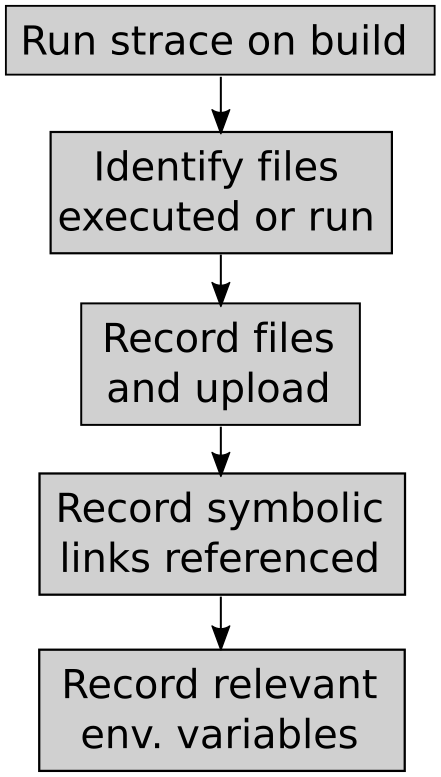
\includegraphics[width=\columnwidth]{duxtrace}
\caption{The steps to trace a build with Dux.}
\end{figure}

At the heart of the tool is a call to \texttt{strace}, which writes to a temporary file. We have \texttt{strace}
record calls to the \texttt{open}, \texttt{execve}, \texttt{readlink}, and \texttt{stat} system calls,
which are the relevant
ones for our purposes: \texttt{open} because any necessary configuration files that building tools use will
have to be opened to be read (it is sufficient to see which ones are opened without logging any of the
calls to \texttt{read}); \texttt{execve} because build managers generally delegate different build steps by
executing the necessary programs (such as compilers or shell scripts); \texttt{readlink} to ensure that we
properly reproduce the directory structure of dependencies by tracking symbolic links; and \texttt{stat} because
it can be used to check the existence of a file without opening it, and we encountered this issue in practice.
By logging these system
calls, Dux obtains a complete view of the files (both those read for information and executed) relevant to the
build process and thus identifies dependencies.

However, the build process may use information beyond that explicitly stored in configuration files; namely,
many builds rely on environment variables (especially \texttt{PATH}), so Dux must capture those as well
in spite of the fact that \texttt{strace} does not handle environmental variables. At present, Dux uses a
simple heuristic to decide which environmental variables to store in the absence of a trace: it parses
all environmental variables (searching for paths) and matches those paths against those logged by strace,
the intent being to find environmental variables specifying dependencies so that build tools can find them.
In the future, we may take a more robust approach by using another tool such as \texttt{ltrace} to trace
exactly which environmental variables are read during the build process, since environmental variables may
encode information other than paths. Dux also includes a mode to simply create a full copy of the environment
when building.

Once Dux has saved the environmental variables deemed relevant and has a trace of system calls, it parses
the system calls to determine which files should be stored in the configuration and should be uploaded to
the store. Storing a file (or symbolic link) in the configuration means simply adding an entry to the
configuration file (named \texttt{build.dux} by default), the entry consisting of a path to the dependency
and a hash of the contents
(except in the case of symbolic links, which are handled separately).
 Note that we ``relativize'' file paths to avoid overspecifity; namely,
if a file path shares a prefix with the directory in which Dux is being invoked, we convert that path to
a relative path. This heuristic is to avoid having paths in the configuration be overly user-specific, as in the
case where a username forms part of a path; we have found that it is generally easier to reuse path information
across users if the paths are relative to the project directory.

Because we only record \texttt{open}, \texttt{execve}, \texttt{stat} and \texttt{readlink} calls, all the
calls that arise in the recorded trace are potentially relevant. Traces for complex builds can be rather
large, though we manage this by processing each file (especially hashing) only once and applying certain
(optional) heuristics to reduce the workload. One heuristic is to disregard files located in the directory 
where Dux is being invoked, since these are ``project files'' and thus not dependencies of the project. 
Another heuristic is to keep a ``blacklist'' of files that are often read during a build but seldom convey 
relevant information or vary spuriously between machines or setups. By default, the ``blacklist'' consists 
only of \texttt{/proc/meminfo} (which contains information about the hardware's capability), though the 
default blacklist may be expanded to include other low-level files once we have run more builds and seen more
 examples of spurious ``dependencies''; the user may also create a file \texttt{.duxignore} to supplement 
the default blacklist with further files or directories for Dux to ignore when parsing \texttt{strace} output.

Once Dux has parsed the \texttt{strace} output and written the relevant files and symbolic links to
the local configuration file, Dux also uploads the logged dependencies to Google Cloud Storage (in a
bucket specified by the user) for future use. We implement our storage as a ``content-addressable
file system'' by naming files after their hashes, relying on the configuration file to recover
the path information for each file; this way, a user can retrieve the contents of a file simply by 
providing the hash logged in the configuration file---allowing an artifact common to multiple builds to
only be uploaded once. We designed this "backend" to be modular, and implementing a different backing store
(such as one based on a URL or using a different cloud provider's API) only requires implementing
"upload" and "download" operations that take a hash and a target file.

\subsection{Validating and Reproducing a Build}

\begin{figure}
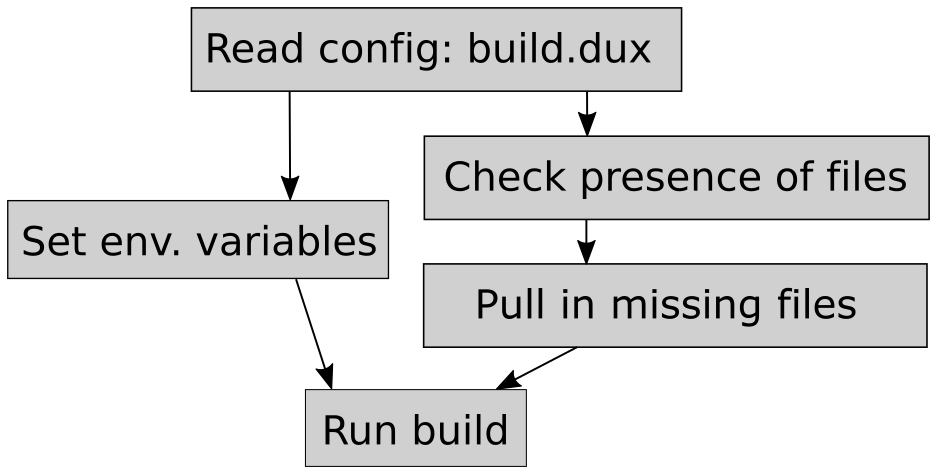
\includegraphics[width=\columnwidth]{duxcheck}
\caption{The steps to replaying a build with Dux.}
\end{figure}

Reproducing a build is essentially the inverse process of that described above. Given a configuration file,
Dux checks that the environmental variables described within are set appropriately and checks that every
file listed in the configuration actually exists. If a file is missing, Dux pulls it in from the backing store
using the hash in the configuration file. If a file is present but has a different hash from that
in the configuration, Dux warns the user but does not retrieve the file from the backing store, since the file
could potentially contain important or system-specific information that is not safe to overwrite. For now,
this is a safe heuristic; in the future, we suspect that it may be necessary to improve our sandboxing to permit
us to safely overwrite arbitrary files. At this stage, Dux also creates any symbolic links that aren't present
on the target machine.

Once Dux has validated its configuration, the build may be run. Dux provides an option to do this itself, spawning
a subprocess with the appropriate environment. Alternatively, Dux can be run in a mode that downloads files,
creates symbolic links, and prints the values of differing environment variables. This second mode allows the user
to inspect the configuration before actually executing the build (which is especially helpful for debugging!).

\section{Evaluation}

To evaluate our prototype of Dux, we used it to reproduce builds for two programs: a simple, UNIX-like shell and
CIL (the C Intermediate Library)\footnote{\url{https://github.com/cil-project/cil}}, an abstraction of C programs
that permits developers of static analyses to more easily reason about C programs. The simple shell was written in
C and built using Make. Its only dependency is on the system's \texttt{readline} library, which is already
present on most UNIX systems. Though this test is not very interesting on its own, it allowed us to test Dux in
a variety of configurations and write simple integration tests\footnote{\url{https://travis-ci.org/kelloggm/dux}}
that demonstrate that Dux behaves as expected in very simple cases.

To test that Dux is capable of building larger-scale projects, we tested it on CIL. CIL is a reasonably-sized
project: it contains about 120,000 lines of mostly OCaml and C code. It has a number of external dependencies,
including on OCaml itself (along with utility tools like \texttt{opam} and \texttt{ocamlfind}), as well as on
various C compilers. It builds using the \texttt{./configure \&\& make \&\& make install} style common to UNIX
utilities. Initially, we had difficulty getting Dux to reproduce builds of CIL. After adding support for symbolic
links, \texttt{stat}, and environment variables, we were able to successfully get Dux to reproduce a build of CIL.
We performed this experiment on a copy of the UW HomeVM for Autumn, 2017; when repeating the build, we deployed
a new copy of the VM (i.e. the underlying OSes were identical). However, it is worth noting that we were unable
to reproduce the build unless the build that was traced started in a fresh copy of the repository, because
configure performs a great deal of first-time setup that Dux fails to capture in subsequent builds (because it
does not happen). Mitigating this issue is future work.

\begin{table}
\begin{center}
\begin{tabular}{ |c|c|c| }
 \hline
 Project & Lines of Code & Files \\ \hline \hline
 shell.c & 165 & 2 \\ \hline
 CIL & 121740 & 952 \\
 \hline
\end{tabular}
\caption{The sizes of the two programs we used to test that Dux can build projects. Dux was able to repeatedly
build both projects.}
\end{center}
\end{table}

\section{Limitations and Future Work}

Dux takes a rather reductive view of the build process, considering only the particular files that are read
and programs that are executed in one build on one system. As such, there are some dimensions to building that
Dux may fail to capture, such as logic that branches on different system configurations or present tools (e.g.,
having different possible builds depending on whether GCC or Clang is present on the system). In the case of
a build supporting different possible configurations, Dux may incorrectly label a machine as lacking proper
configuration when, in fact, the build may very well succeed on that machine using one of the alternatives. 
It is not obvious how Dux can be modified to address this; a user would have to keep around different configuration 
files for different possible builds and know which Dux configuration to pass around appropriately. That said, this 
is a possible avenue of future work. One possible scheme could include the production of a Dux configuration 
file for each supported operating system by the developers, and a check within Dux of which OS it is operating 
on. Dux could then choose the appropriate configuration file and proceed with the build.

Since Dux uploads dependencies without regard for their particular use, this may also lead to broken builds 
if it is applied on a system different from the one that was used to produce the configuration for a build, 
since Dux will pull in binaries that might have been compiled for a different system. A modification that
might hedge against this case would be keeping hashes of system metadata in configurations and knowing
that an executed binary from another system should likely not be pulled in to a different one. It may also
be possible for Dux to store more information in the cloud---for instance, Dux could keep track of the names
of dependencies and what kind of system they came from, and try to substitue appropriate ones if the build does
not work the first time. So, for instance, if the configuraton file calls for \texttt{gcc} generated an OSX machine,
but the target machine is running Ubuntu, Dux could search in its cloud for a copy of \texttt{gcc} that was
generated on Ubuntu. While our prototype does not currently attempt to implement this feature, a complete
implementation of Dux probably would.

A key limitation of our current prototype is: how does Dux deal with
change, either in the environment or in the code it is building? We view building
the version of Dux we described here as the first step towards an adaptive
build system that can repair build scripts when they fail, using techniques
from the automated program repair literature. Existing program repair techniques
suffer from high false positive rates, in large part due to the unstructured
nature of the problem---with only a few (hundred? thousand?) test cases, it is
difficult to model all the correct behavior of a large C program~\cite{genprogisbadrinard}.
By contrast, the structured nature of a build configuration file and the relatively
small size of the change set make build script repair an attractive domain for
automated repair tools. By combining a tool like Dux with a build script repair
system, one can imagine a build tool that can correctly deploy software even in
the face of different dependency requirements or a different platform automatically,
making deploying software in new environments a much simpler process.

\section{Related Work}

Several modern build systems include a dependency management strategy. Tools like
Maven~\cite{Maven}, Gradle~\cite{Gradle}, Bazel~\cite{blaze}, or Buck~\cite{buck}
are primarily systems for building and testing software, but each includes the
ability to specify dependencies manually in some kind of configuration file.
Ivy~\cite{Ivy} is exclusively a dependency management tool, but still requires
a manually written configuration file.
Unlike Dux's configuration files, which are automatically generated, the configuration
files for these tools use domain-specific languages that developers have to learn,
write, and maintain. Some tools (such as Bazel) also include sandboxing tools
that force the build to only use dependencies explicitly specified in the
configuration file. The Homebrew package manager for Mac OSX also includes
a system called "bottles", which resemble Dux configuration entries\cite{homebrew}.
Each bottle, like a dependency in Dux, represents a binary that can be downloaded
from a central server, and Homebrew includes some automated tooling to help
developers create the scripts used to download dependencies. However,
Homebrew is focused entirely on deploying applications to a single hardware/software
combination, and lacks the flexibility and generality of Dux.

Most recent advances in build technology have come from industry, not from
academia. Adams and McIntosh breifly cover build systems in their survey of
release engineering~\cite{adams2016modern}, in an effort to urge academics to
pay more attention to the work going on in industry. Cox et al. examined how
to prioritize updating dependencies, but did not attempt to fix build issues~\cite{cox2015measuring}.
McIntosh et al. built a classifier to determine when changes to the build
system would be necessary based on the changes introduced to source code~\cite{mcintosh2014mining}.
Seo et al. performed an empirical study at Google, and determined that more
than 50\% of build breakages were caused by dependency errors~\cite{googlebuilderrors}.
This is especially motivating for our work, since Google's Bazel build system
is considered the industry standard---and dependency issues are their most
common build error.

\section{References}

\begingroup
\renewcommand{\section}[2]{}%

% The following two commands are all you need in the initial runs of
% your .tex file to produce the bibliography for the citations in your
% paper.
\bibliographystyle{plain}
\bibliography{genprog-bib/merged}
% You must have a proper ``.bib'' file
% and remember to run:
% latex bibtex latex latex
% to resolve all references
%
% ACM needs 'a single self-contained file'!
%
\endgroup

\end{document}
